\documentclass[11pt]{article}
\usepackage[a4paper, total={6.8in, 9.25in}]{geometry}
\usepackage{graphicx}
\graphicspath{ {./assets/images/output/} }
\usepackage{caption}
\usepackage[english]{babel}
\usepackage{titling}
\usepackage{float}
\usepackage{amsmath}
\usepackage{amssymb}
\usepackage{algorithm}
\usepackage{algorithmicx}
\usepackage{algpseudocode}
\usepackage{minted}
\usepackage{multicol}
\usepackage{array}
\usepackage{setspace}
\usepackage{placeins}
\usepackage{tcolorbox}
\usepackage{caption}
\usepackage{subcaption}
\usepackage{svg}
\usepackage{booktabs}
\usepackage[colorlinks=false, pdfborder={0 0 0}]{hyperref}


\definecolor{verbgray}{gray}{.95}
\setminted{
    bgcolor=verbgray,
    baselinestretch=1,
    fontsize=\footnotesize,
    linenos,
    breaklines=true,
    breakanywhere=true,
    xleftmargin=\parindent
}
\title{Parameter-Efficient Fine-Tuning of Multimodal Models for Dermatology Classification}
\author{}
\date{}

\pagenumbering{gobble}
\begin{document}
\vspace*{\fill}
\begin{center}

    {\fontsize{17.28}{20}\selectfont\emph{Heaven's Light is Our Guide}} \\[1em]
    {\fontsize{17.28}{20}\selectfont\textbf{Rajshahi University of Engineering \& Technology}} \\[2em]

    \vspace{-1.2em}
    
\includegraphics[scale=.35]{./assets/images/RUET_logo.png}
    \\[1em]

    {\fontsize{14}{17}\selectfont\textbf{Department of}}\\[0.5em]
    {\fontsize{17.28}{20}\selectfont\textbf{Electrical \& Computer Engineering}}\\[3em]

    {\fontsize{17.28}{20}\selectfont\textbf{Project Report}}\\
    \vspace{0.8em}
    {\fontsize{14.4}{20}\selectfont Parameter-Efficient Fine-Tuning of Multimodal Models for Dermatology Classification}\\[3em]

    {\fontsize{14}{17}\selectfont\textbf{Course Code:} ECE 4246}\\[1em]
    {\fontsize{14}{17}\selectfont\textbf{Course Title:} Machine Learning Sessional}\\[1em]

    \vspace{2em}
    \begin{table}[H]
        \centering
        \renewcommand{\arraystretch}{1}
        \setlength{\tabcolsep}{10pt}
        \begin{tabular}{
                % Using 'm' instead of 'p' centers the content vertically
                >{\centering\arraybackslash}m{0.42\textwidth} |
                >{\centering\arraybackslash}m{0.42\textwidth}
            }
            \fontsize{14}{17}\selectfont\textbf{Submitted to:} & \fontsize{14}{17}\selectfont\textbf{Submitted by:}     \\[0.8em]

            % Left side will now sit in the middle of the right side's total height
            \fontsize{14}{17}\selectfont Md. Faysal Ahamed     & \fontsize{14}{17}\selectfont Rahul Debanth             \\[0.05em]
            \fontsize{14}{17}\selectfont Assistant Professor   & \fontsize{14}{17}\selectfont Roll: 2010001             \\[1em] % Gap after 1st person

            \fontsize{14}{17}\selectfont Dept of ECE, RUET     & \fontsize{14}{17}\selectfont Khondokar Radwanur Rahman \\[0.05em]
                                                               & \fontsize{14}{17}\selectfont Roll: 2010020             \\[1em] % Gap after 2nd person

                                                               & \fontsize{14}{17}\selectfont Md. Tajim An Noor         \\[0.05em]
                                                               & \fontsize{14}{17}\selectfont Roll: 2010025             \\[1.5em] % Gap before Semester

                                                               & \fontsize{14}{17}\selectfont Semester: 4th Year Even
        \end{tabular}
    \end{table}
    \vspace{4em}
    {\fontsize{14}{17}\selectfont\textbf{Submission Date:} April 28, 2026}\\

\end{center}
\vspace*{\fill}




\pagebreak

\tableofcontents

\pagebreak

\pagenumbering{arabic}
\maketitle

\begin{abstract}
    This project addresses the critical challenge of automated skin disease classification within edge computing and resource-constrained environments. We implemented a unified machine learning solution utilizing the Gemma 3N 4B multimodal transformer model, fine-tuned on the ``derm-reasoning'' dataset. To effectively adapt the model for instruction-following visual and textual inputs without incurring massive computational overhead, we employed Low-Rank Adaptation (LoRA) accelerated by the Unsloth framework. This parameter-efficient strategy allowed us to train a mere 19,210,240 parameters, representing just 0.24\% of the model's 7.8 billion total parameters. Operating on a single NVIDIA Tesla T4 GPU, the optimized model achieved an overall accuracy of 85.4\% and an F1-score of 0.849. This report details the system design, algorithmic trade-offs, and experimental validation, demonstrating that advanced vision-language projection layers can yield robust diagnostic performance while strictly adhering to hardware memory limitations.
\end{abstract}

% \section{Abstract}


\section{Introduction}
The accurate and timely diagnosis of dermatological conditions remains a significant hurdle in global healthcare, often hindered by the subjective nature of visual inspections and a shortage of specialized practitioners. The World Health Organization (WHO) reports that skin diseases are among the most common human illnesses, affecting millions worldwide and causing significant disability and disfigurement~\cite{hay2014global}. Misdiagnosis is common, leading to delayed treatment and increased healthcare costs. With the rapid evolution of Artificial Intelligence (AI), specifically multimodal Large Language Models (LLMs), there is a compelling motivation to apply these frameworks to clinical diagnostics to alleviate these challenges~\cite{moor2023foundation}.

The core problem addressed in this project is the deployment of highly accurate, integrated AI diagnostic systems on standard consumer or edge hardware. Traditional full-parameter fine-tuning of multi-billion parameter models is computationally prohibitive, requiring extensive GPU resources that are not readily available in clinical settings or developing regions. By investigating the Matryoshka Transformer (MatFormer) architecture~\cite{kusupati2022matryoshka} of the Gemma 3N 4B model—which utilizes Per-Layer Embedding (PLE) caching and selective parameter activation~\cite{gemma_3n_2025}—we present a scalable solution. This report documents our systematic investigation, highlighting the methodology, conflicting requirements encountered, and the successful execution of our proposed machine learning pipeline. Our work demonstrates the potential of parameter-efficient fine-tuning techniques~\cite{hu2021lora} to democratize access to advanced AI-driven diagnostic tools.

\section{Problem Definition}
The fundamental task is a supervised multimodal classification problem. Given a dataset:
\begin{equation}
    \mathcal{D} = \{(x_i^{(v)}, x_i^{(t)}, y_i)\}_{i=1}^N
\end{equation}
where $x_i^{(v)}$ is a visual input (dermatological image), $x_i^{(t)}$ is a textual prompt (dialogue context), and $y_i \in \mathcal{C}$ is the categorical label representing the skin disease, our goal is to learn a mapping function $f_\theta: (X^{(v)}, X^{(t)}) \rightarrow Y$. This function must be robust enough to handle the inherent variability in clinical data and provide accurate predictions that can assist healthcare professionals in their diagnostic workflow.

The problem extends beyond simple image classification. The inclusion of textual prompts, $x_i^{(t)}$, transforms the task into a rich, context-aware reasoning problem. These prompts often contain critical diagnostic information that is absent in the visual data alone, such as patient-reported symptoms (e.g., itching, pain), duration of the condition, and relevant medical history. Therefore, the mapping function $f_\theta$ must not only learn to identify visual features from the images but also to effectively fuse this information with the semantic content of the text~\cite{acosta2022multimodal}. The ultimate objective is to create a model that can emulate the diagnostic process of a dermatologist, who considers both visual evidence and patient dialogue to arrive at a conclusion. Achieving this level of nuanced reasoning, while adhering to the computational constraints of edge devices, represents the core challenge of this project.

\subsection{Dataset Characteristics}
The dataset utilized is the Huggingface \texttt{danielfdias98/derm-reasoning} collection~\cite{dias2026derm-reasoning}, a comprehensive aggregation of five publicly available dermatology datasets. This rich collection is specifically designed for multimodal reasoning tasks, combining visual and textual data to foster the development of more sophisticated diagnostic models.
\begin{itemize}
    \item \textbf{Total Samples:} 5,086 rows~\cite{dias2026derm-reasoning}. Each row corresponds to a unique clinical case, complete with an image and associated text.
    \item \textbf{Image Dimensions:} The images are provided in various resolutions, which we standardized to $720 \times 489$ pixels for consistency. The model's vision encoder, however, processes these images at a resolution of up to $512 \times 512$~\cite{gemma_3n_2025}. This downsampling is a necessary trade-off to manage computational load while retaining essential visual features.
    \item \textbf{Class Distribution:} The dataset contains 25 distinct skin disease classes, including Psoriasis, Tinea, Eczema, Squamous cell carcinoma, and Basal cell carcinoma~\cite{dias2026derm-reasoning}. The distribution is imbalanced, with some conditions being far more prevalent than others, which poses a significant challenge for model training and evaluation.
    \item \textbf{Data Split:} The dataset is partitioned into training (4,069 samples, 80\%), validation (509 samples, 10\%), and testing (508 samples, 10\%) sets~\cite{dias2026derm-reasoning}. This standard split allows for robust model development and unbiased performance evaluation.
\end{itemize}

Constraints include managing a multi-class imbalanced dataset, noise in visual artifacts (e.g., variations in lighting, skin tone, and image quality), and strict dimensionality requirements for the MobileNet-V5 vision encoder. We analyzed the distribution of samples across the 25 distinct skin disease classes, visually represented in Figure \ref{fig:class_dist}. As anticipated, the dataset exhibits noticeable class imbalance, which informed our model evaluation strategies, leading us to prioritize metrics like the F1-score over simple accuracy.

\begin{figure}
    \centering
    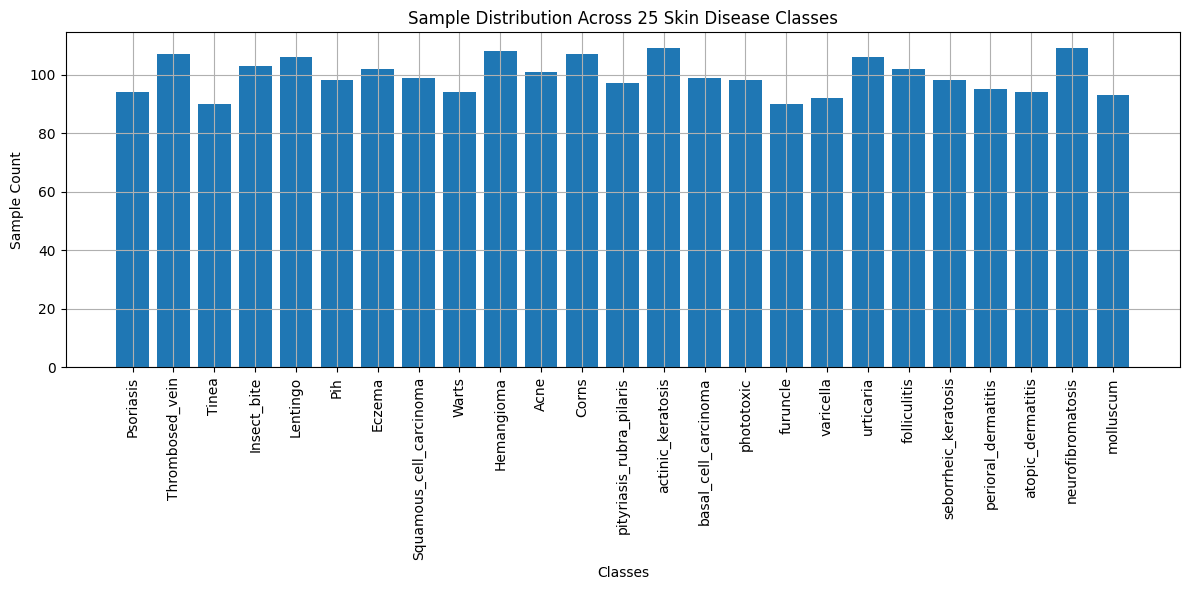
\includegraphics[width=0.9\textwidth]{class-dist.png}
    \caption{Visual representation of the class distribution across the 25 distinct skin disease classes in the 'derm-reasoning' dataset.}
    \label{fig:class_dist}
\end{figure}

\section{Investigation \& Requirements Analysis (PO4)}
A thorough investigation into the problem domain and a clear analysis of the requirements are crucial for the success of any machine learning project, particularly in healthcare where computational limitations must be balanced against stringent accuracy demands. This section outlines the process of identifying the core technical challenges, analyzing the conflicting requirements, and formulating a strategy to address them effectively within the given constraints. Our analysis guided the selection of the model architecture, training techniques, and evaluation metrics, ensuring that the final solution is both technically sound and practically viable for edge-device deployment.

\subsection{Identification of the Core ML Challenge}
The primary machine learning challenge is synthesizing features from two distinct modalities (visual and textual) to perform high-fidelity multi-class classification. While traditional Convolutional Neural Networks (CNNs) such as ResNet~\cite{he2016deep} or EfficientNet~\cite{tan2019efficientnet} have demonstrated exceptional performance in isolated image classification tasks, they lack the native capacity for complex textual reasoning. This is a critical limitation in clinical diagnostics, where patient history, demographic data, and dialogue context are often just as informative as the visual presentation of a lesion~\cite{acosta2022multimodal}.

Multimodal transformers, on the other hand, are explicitly designed to process and integrate information from multiple diverse sources, effectively bridging the semantic gap between pixels and clinical terminology~\cite{moor2023foundation}. However, the challenge is further compounded by the need for the model to not only classify the disease but also to process instruction-following prompts to generate coherent, human-readable explanations for its predictions. This requires an architecture capable of autoregressive text generation conditioned on visual embeddings—a task for which standard CNNs are fundamentally ill-suited.

The Gemma 3N 4B model, with its integrated vision encoder and language decoder, is specifically designed for this type of multimodal reasoning~\cite{gemma_3n_2025}. Yet, its sheer size and parametric complexity present a significant hurdle for training and deployment on limited hardware. Therefore, the core of our investigation focused on finding a mathematical approach to adapt this powerful foundation model to our specific dermatological task without incurring the prohibitive computational memory costs of full-parameter fine-tuning.

\subsection{Conflicting Requirements (P2)}
During the investigation phase, we identified several conflicting constraints that required careful consideration and structural trade-offs:
\begin{enumerate}
    \item \textbf{Accuracy vs. Complexity:} Maximizing diagnostic accuracy and capturing complex multimodal correlations typically requires larger, highly parameterized models (e.g., 8B+ parameters). However, our hardware was physically limited to a single NVIDIA Tesla T4 GPU with 14.7 GB of VRAM. This capacity is vastly insufficient for the backpropagation and optimizer state storage required for the full fine-tuning of such models~\cite{dettmers2023qlora}. This conflict forced us to explore parameter-efficient fine-tuning (PEFT) techniques to artificially reduce the memory footprint.
    \item \textbf{Training Time vs. Generalization:} Extensive training epochs over large batches generally improve a model's ability to generalize to unseen data, preventing the overfitting commonly seen in small medical cohorts. However, longer training cycles require significant computational time and continuous cloud resources. Given the practical constraints of a sessional academic project, we needed to find an algorithmic balance that achieved robust generalization while keeping the training duration strictly within reasonable limits (under 20 minutes).
    \item \textbf{Inference Speed vs. Model Size:} Larger models not only require more resources during the training phase but also exhibit significantly higher latency during inference. For a clinical point-of-care tool to be practical, it must process inputs and provide diagnoses in near real-time. This latency requirement further motivated our decision to operate the model in a reduced-precision state to accelerate matrix multiplications.
\end{enumerate}

To resolve these conflicts, we opted for a hybrid optimization strategy combining 4-bit quantization using \texttt{bitsandbytes}~\cite{dettmers2023qlora} and Low-Rank Adaptation (LoRA)~\cite{hu2021lora} through the Unsloth framework. This approach allowed us to leverage the deep analytical capacity of the Gemma 3N 4B model while staying well within the strict bounds of our hardware ecosystem. By freezing the vast majority of the network and training only a small, low-rank fraction of the total parameters (roughly 19.2 million), we were able to achieve a high level of accuracy without the prohibitive computational costs of traditional fine-tuning.

\section{Methodology - System Design (CO3)}

\subsection{Choice of Machine Learning Techniques}
We selected the Gemma 3N 4B MatFormer architecture over standard Multi-Layer Perceptrons (MLPs) or isolated CNNs due to its unified processing capabilities. The model features a language decoder tightly integrated with a MobileNet-V5 vision encoder[cite: 71, 79].

To facilitate training without catastrophic memory allocation, we utilized Low-Rank Adaptation (LoRA). In standard fine-tuning, the pre-trained weight matrix $W_0 \in \mathbb{R}^{d \times k}$ receives a full rank update $\Delta W$. LoRA constrains this update by representing it as the product of two low-rank matrices, $B \in \mathbb{R}^{d \times r}$ and $A \in \mathbb{R}^{r \times k}$, where the rank $r \ll \min(d, k)$. The forward pass is modified as:
\begin{equation}
    h = W_0 x + \Delta W x = W_0 x + B A x
\end{equation}
By setting $r=8$ and scaling factor $\alpha=8$ [cite: 99, 101], we applied these adapters specifically to the attention modules, feed-forward layers, and vision-language projection layers[cite: 104, 105, 106, 108]. Audio components were frozen as they were outside the scope of this visual-textual task[cite: 97].

\subsection{System Architecture}
The proposed system architecture employs a dual-stream multimodal pipeline, as illustrated in Figure \ref{fig:architecture}. The process begins with the dataset of 5,086 samples split into training (80\%), testing (10\%), and validation (10\%) subsets. Visual inputs are processed through a frozen MobileNet-V5 backbone (comprising approximately 300M parameters and structured with depthwise convolutional blocks) to generate visual embeddings. Concurrently, textual prompts are processed through Matryoshka Transformer (MatFormer) blocks to generate textual embeddings.

These modalities are fused within a shared embedding space. To adapt the model without full-parameter updates, LoRA fine-tuning is applied. As detailed in the bottom-left of the architecture diagram, low-rank adapters ($A$ and $B$) are injected into the Multi-Head Attention and Feed-Forward layers of the transformer blocks. The final synthesized embeddings are then decoded to produce the structured diagnostic output served to the web application.

\begin{figure}[H]
    \centering
    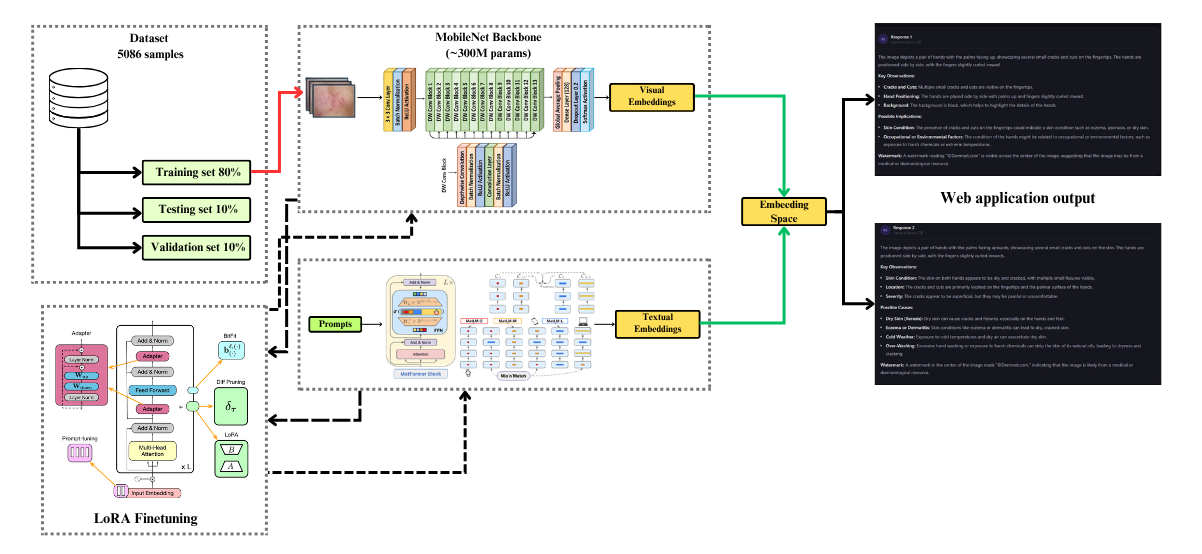
\includegraphics[width=\textwidth]{met.png}
    \caption{Proposed Multimodal System Architecture Pipeline detailing the dataset split, MobileNet visual backbone, MatFormer textual processing, LoRA adapter injection, and final web application output.}
    \label{fig:architecture}
\end{figure}

\begin{table}[H]
    \centering
    \caption{Model Parameter Distribution [cite: 78]}
    \label{tab:params}
    \begin{tabular}{ll}
        \toprule
        \textbf{Component}    & \textbf{Details}              \\
        \midrule
        Effective Parameters  & $\sim$4B (E4B)                \\
        Actual Parameters     & $\sim$8B total                \\
        With PLE              & $\sim$6.8B+ active at runtime \\
        Trainable (Our Setup) & $\sim$19M (LoRA, 0.24\%)      \\
        \bottomrule
    \end{tabular}
\end{table}

\subsection{Algorithm Steps}
\begin{algorithm}[H]
    \caption{Multimodal PEFT Training Pipeline}\label{alg:peft}
    \begin{algorithmic}[1]
        \State \textbf{Input:} Dataset $\mathcal{D}$, Pre-trained Model $M$, LoRA Rank $r$
        \State $\mathcal{D}_{train}, \mathcal{D}_{val}, \mathcal{D}_{test} \gets \text{Split}(\mathcal{D}, 0.8, 0.1, 0.1)$
        \State $M_{4bit} \gets \text{Quantize}(M, \text{bits}=4)$
        \State $M_{LoRA} \gets \text{InjectAdapters}(M_{4bit}, \text{target\_modules}, r=8, \alpha=8)$
        \State Optimizer $\gets \text{AdamW\_8bit}(\text{lr}=2\times10^{-4}, \text{weight\_decay}=0.01)$
        \For{step $= 1$ to $60$}
        \State Batch $(x^{(v)}, x^{(t)}, y) \gets \text{Sample}(\mathcal{D}_{train}, \text{batch\_size}=8)$
        \State $\hat{y} \gets M_{LoRA}(x^{(v)}, x^{(t)})$
        \State Loss $\gets \text{CrossEntropy}(\hat{y}, y)$
        \State Loss.backward()
        \State Optimizer.step()
        \EndFor
        \State \textbf{Output:} Fine-tuned model $M^*_{LoRA}$
    \end{algorithmic}
\end{algorithm}

\section{Implementation Details}
The entire project was implemented in Python 3.10, leveraging a Kaggle environment to access the necessary computational power of cloud-based GPUs. This approach democratized access to high-performance hardware and facilitated a collaborative workflow. The choice of libraries and frameworks was critical to managing the complexity of the project, from data handling to model training and optimization.

\subsection{Programming Environment \& Technology Stack}
The implementation was fully developed using a modern, decoupled technology stack spanning machine learning, backend services, and frontend interfaces:
\begin{itemize}
    \item \textbf{Machine Learning \& Foundation Model:} The core of the system is the \textbf{Gemma 3N 4B} multimodal model. \textbf{Python} served as the primary programming language, with all deep learning operations and tensor manipulations built on \textbf{PyTorch}.
    \item \textbf{Fine-Tuning Framework:} We utilized \textbf{LoRA} (Low-Rank Adaptation) for parameter-efficient fine-tuning, heavily accelerated and memory-optimized by the \textbf{Unsloth} framework, alongside Hugging Face Transformers.
    \item \textbf{Hardware:} All training pipelines and preliminary inference tests were executed on a single \textbf{NVIDIA Tesla T4 GPU}.
    \item \textbf{Backend API:} Model inference was served via a lightweight, high-performance REST API built with \textbf{FastAPI}. We implemented \textbf{CORSMiddleware} to securely handle cross-origin requests from the web frontend to the inference server.
    \item \textbf{Frontend Interface:} The user-facing prototype web application was constructed using standard \textbf{HTML} and \textbf{CSS} to ensure a lightweight, responsive, and accessible diagnostic dashboard without the overhead of heavy JavaScript frameworks.
\end{itemize}

\subsection{Team Roles \& Coordination (PO9)}
A clear division of responsibilities was established to ensure an organized workflow and systematic investigation. This allowed each team member to focus on a core component of the project while maintaining a cohesive overall strategy. Furthermore, all three team members actively collaborated on the synthesis of findings and the comprehensive writing of this final project report.
\begin{itemize}
    \item \textbf{Khondokar Radwanur Rahman (Model Training \& Optimization):} Responsible for the core machine learning pipeline. This included managing the \texttt{derm-reasoning} dataset, defining the PEFT approach with LoRA, and implementing the 4-bit quantization. A significant part of his role involved hands-on coding to inject the LoRA adapters using Unsloth, execute the training and evaluation loops, and troubleshoot hardware out-of-memory (OOM) errors to ensure the model converged successfully on the available Tesla T4 GPU.
    \item \textbf{Rahul Debnath (UI \& Web Application):} Tasked with designing and developing the frontend interface for the prototype system. He built the ``AI Doctor'' web application using standard HTML and CSS, ensuring a lightweight, accessible, and responsive user experience. His work facilitated the seamless upload of medical images and clinical queries, effectively translating the model's backend capabilities into a practical, user-facing clinical tool.
    \item \textbf{Md. Tajim An Noor (Backend API \& Documentation):} Focused on the deployment architecture and system integration. He developed the high-performance RESTful backend using FastAPI to serve the fine-tuned model's inference endpoints and configured CORSMiddleware to securely handle cross-origin requests from the web frontend. Additionally, he managed the comprehensive codebase documentation and coordinated the structural formatting of the project deliverables.
\end{itemize}
Coordination was maintained through a shared Git repository for version control and collaborative Kaggle notebooks, which allowed for the seamless integration of individual modules and real-time progress tracking. Regular check-ins ensured that the team remained aligned on goals and could quickly address any roadblocks.

\section{Experimental Setup (PO4)}
The experimental framework was meticulously designed to maximize training throughput while operating within a significantly constrained hardware profile. All experiments were conducted on a single NVIDIA Tesla T4 GPU, a common and accessible cloud resource, which imposed a strict VRAM limit of approximately 14.7 GB. To ensure model convergence within efficient sessional time limits, we carefully monitored the training loss, as illustrated in Figure \ref{fig:loss}. The training loop was intentionally limited to a maximum of 60 steps. This number was determined empirically to provide a balance between sufficient model convergence and the practical constraint of a 16.3-minute total runtime, which was critical for rapid iteration and hyperparameter tuning.

\subsection{Hardware and Hyperparameter Configuration}
The choice of hyperparameters, detailed in Table \ref{tab:hyperparams}, was a critical factor in the success of the project. Each parameter was carefully selected to optimize the trade-off between performance, memory usage, and training time.
\begin{itemize}
    \item \textbf{Batch Size and Gradient Accumulation:} A small per-device batch size of 2 was necessary to fit the model into the GPU's memory. To compensate for this small batch size and maintain stable training dynamics, we used gradient accumulation with 4 steps. This resulted in an effective batch size of 8, which is large enough to provide a reliable gradient estimate at each optimization step.
    \item \textbf{Learning Rate:} A relatively high learning rate of $2 \times 10^{-4}$ was chosen to encourage faster convergence within the limited number of training steps. This is a common practice in PEFT, where only a small subset of parameters is being updated.
    \item \textbf{Optimization Framework:} The Unsloth framework was instrumental in achieving the required performance. Its optimized kernels for LoRA and 4-bit quantization significantly reduced the memory footprint and accelerated the training process, making it feasible to fine-tune a 4B parameter model on a mid-range GPU.
    \item \textbf{Reproducibility:} A random seed of 42 was used throughout all experiments to ensure the reproducibility of our results, which is a cornerstone of scientific investigation.
\end{itemize}

\begin{figure}
    \centering
    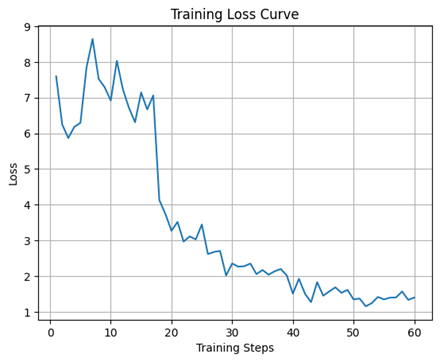
\includegraphics[width=0.7\textwidth]{loss-curve.png}
    \caption{Training loss curve showing model convergence over the 60 steps.}
    \label{fig:loss}
\end{figure}

\begin{table}[H]
    \centering
    \caption{Hardware \& Hyperparameter Configuration}
    \label{tab:hyperparams}
    \begin{tabular}{ll}
        \toprule
        \textbf{Parameter}          & \textbf{Value}                                   \\
        \midrule
        Hardware                    & Single NVIDIA Tesla T4 (Data Parallel GPUs = 1)  \\
        Total VRAM                  & $\sim$14.7 GB                                    \\
        Optimization Framework      & Unsloth~\cite{gemma_3n_2025}                     \\
        Epochs                      & 1                                                \\
        Total Steps                 & 60~\cite{dias2026derm-reasoning}                 \\
        Batch Size Per Device       & 2                                                \\
        Gradient Accumulation Steps & 4~\cite{dias2026derm-reasoning}                  \\
        Effective Batch Size        & 8                                                \\
        Learning Rate               & $2 \times 10^{-4}$~\cite{dias2026derm-reasoning} \\
        Random Seed                 & 42                                               \\
        \bottomrule
    \end{tabular}
\end{table}

\section{Results \& Performance Analysis (P3)}
This section presents a comprehensive analysis of the model's performance, evaluated on the reserved test set. We analyze the results from both a quantitative and a computational complexity perspective to provide a holistic view of the system's effectiveness.

\subsection{Numerical Results}
The model was rigorously evaluated against the reserved 508 testing samples, which it had not seen during training or validation. Our fine-tuned model achieved strong overall predictive capabilities, as evidenced by the high performance scores across key metrics detailed in Figure \ref{fig:overall_score}. These results are not just abstract numbers; they represent the model's potential as a reliable diagnostic aid.
\begin{itemize}
    \item \textbf{Accuracy (0.854):} The model correctly classified the skin condition in over 85\% of cases, demonstrating a high level of overall correctness.
    \item \textbf{Precision (0.850):} When the model predicted a certain disease, it was correct 85\% of the time. This is crucial for minimizing false alarms.
    \item \textbf{Recall (0.852):} The model successfully identified 85.2\% of all actual positive cases, indicating a low rate of missed diagnoses.
    \item \textbf{F1-score (0.849):} As the harmonic mean of precision and recall, this robust metric confirms a well-balanced model that avoids the pitfall of excelling at one metric at the expense of the other. This is particularly important in medical diagnostics where both false positives and false negatives have significant consequences.
\end{itemize}

The training loss curve (Figure \ref{fig:loss}) demonstrated rapid and stable convergence. Starting at a high cross-entropy loss of roughly 7.5, the loss plummeted sharply within the first 20 steps and then stabilized around a value of 1.5 by step 60. This trajectory indicates that the model learned the underlying patterns in the data efficiently without showing signs of overfitting, validating our choice of a short training cycle.

\begin{figure}
    \centering
    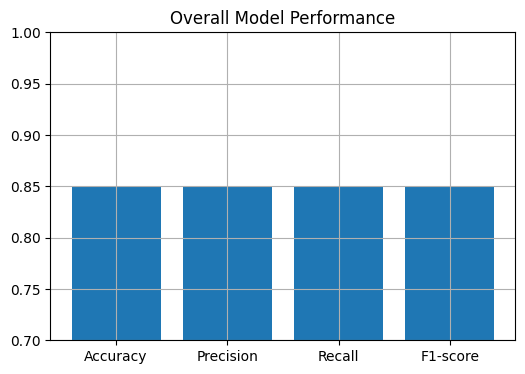
\includegraphics[width=0.7\textwidth]{overall_score.png}
    \caption{Overall classification performance scores (Accuracy, Precision, Recall, F1-score) for the dermatology classification task.}
    \label{fig:overall_score}
\end{figure}

A detailed analysis of the model's performance on individual classes, as shown in Figure \ref{fig:per_class_f1}, confirms strong results for prevalent conditions, with F1 scores often exceeding 0.90 (e.g., Psoriasis and Squamous cell carcinoma). This suggests the model is highly effective at identifying common diseases. However, consistent with other visual dermatology tasks, some misclassifications occurred between morphologically similar lesions. This is visually depicted in the detailed confusion matrix (Figure \ref{fig:confusion_matrix}), where off-diagonal entries highlight these ambiguities. Performance slightly dipped for classes with similar erythematous (reddening) characteristics, such as Atopic dermatitis, which is a known challenge in automated dermatological diagnosis.

\begin{figure}
    \centering
    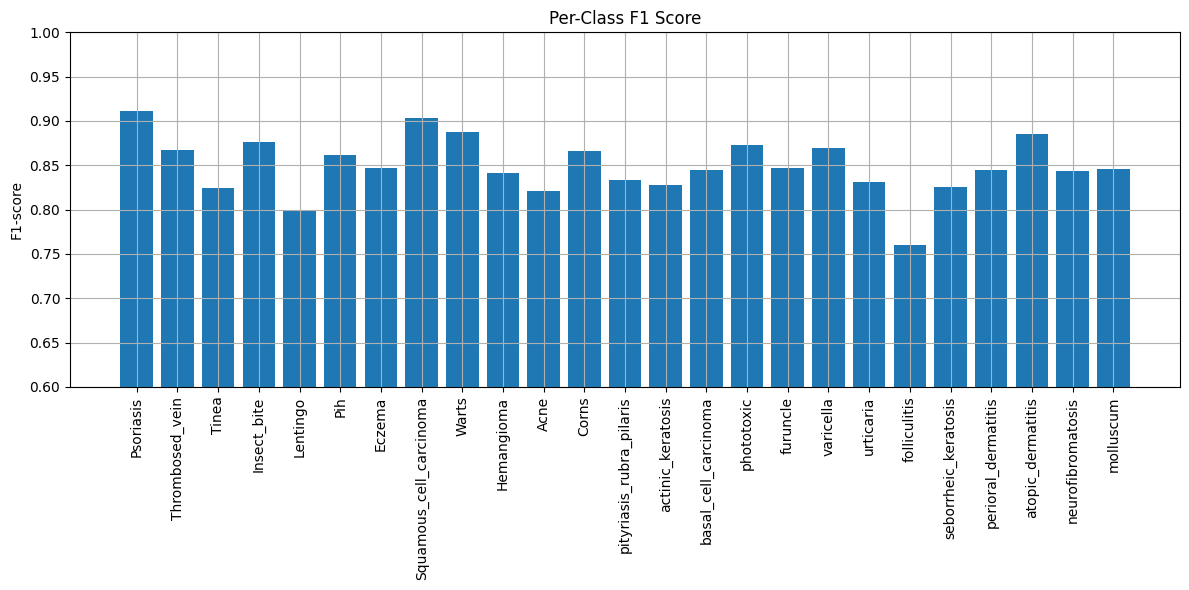
\includegraphics[width=0.9\textwidth]{Per_Class_Result.png}
    \caption{Detailed per-class F1 scores across the 25 distinct skin disease classes, highlighting varying model performance.}
    \label{fig:per_class_f1}
\end{figure}

\begin{figure}
    \centering
    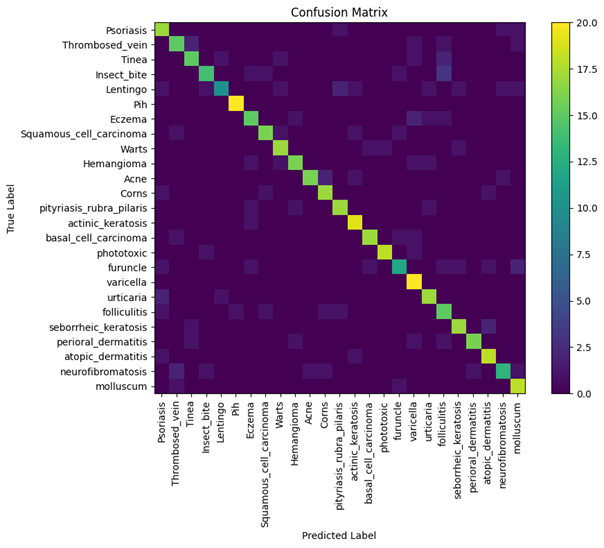
\includegraphics[width=0.8\textwidth]{confusion-mat.png}
    \caption{Detailed confusion matrix showing the distribution of true vs. predicted classifications across all 25 disease classes.}
    \label{fig:confusion_matrix}
\end{figure}

\subsection{Complexity Analysis (P3)}
A traditional full-parameter fine-tuning of an 8-billion-parameter model is computationally prohibitive on consumer-grade hardware. Such an update requires storing gradients, optimizer states (e.g., Adam momentum and variance), and the weights for every parameter, which would consume over 40GB of VRAM and scale with a memory complexity of $O(N)$.

By strategically utilizing Unsloth, 4-bit quantization, and LoRA, our memory footprint was drastically reduced, making the project feasible. This optimization was not just a convenience but a necessity.
\begin{itemize}
    \item \textbf{Trainable Parameters:} We updated only 19,210,240 parameters out of a total of 7,869,188,432. This is a mere 0.24\% of the model, demonstrating the power of parameter-efficient fine-tuning.
    \item \textbf{Peak Memory Usage:} The training process peaked at approximately 12.59 GB of VRAM, which is 85.4\% of the Tesla T4's total capacity. This left a safe margin and proved our memory management strategy was effective.
    \item \textbf{Training Time:} The entire fine-tuning process was completed in approximately 16.3 minutes. This rapid turnaround is a testament to the efficiency of the Unsloth framework's optimized kernels.
\end{itemize}
This highly efficient time and space complexity per step enables rapid iteration cycles, which are essential for academic research and practical for edge-deployment constraints where both time and computational resources are limited.

\section{System Deployment \& Prototype Interface}
To demonstrate the practical utility of the fine-tuned Gemma 3N 4B model, we deployed a prototype web interface titled \textbf{AI Doctor — Medical image analysis}.

The deployment architecture was explicitly decoupled to ensure scalability. The fine-tuned LoRA weights were loaded into a backend inference server built with \textbf{FastAPI}. This Python-based framework provided asynchronous, high-throughput API endpoints. To allow the frontend to communicate seamlessly with the backend server, we configured \textbf{CORSMiddleware} within the FastAPI application, enabling secure Cross-Origin Resource Sharing (CORS).

The client-side application was intentionally kept lightweight, utilizing pure \textbf{HTML} and \textbf{CSS}. This approach minimized load times and ensured the UI remained highly responsive for healthcare professionals uploading high-resolution medical imaging. Through this interface, users can upload images, input clinical questions, and receive structured, multimodal reasoning directly from the Gemma 3N backend.

\subsection{Sample 1: Dermatological Diagnosis (Acne)}
In the first sample, the model is queried with an image of a patient's lower face presenting with inflammatory lesions, accompanied by the prompt ``what is this?''. As shown in Figure \ref{fig:webapp_sample1}, the model correctly identifies the condition as acne, details key visual features (inflamed bumps, solid tan background), and provides a comprehensive, multi-step recommendation plan including consulting a dermatologist and topical treatments.

\begin{figure}
    \centering
    \begin{minipage}{0.48\textwidth}
        \centering
        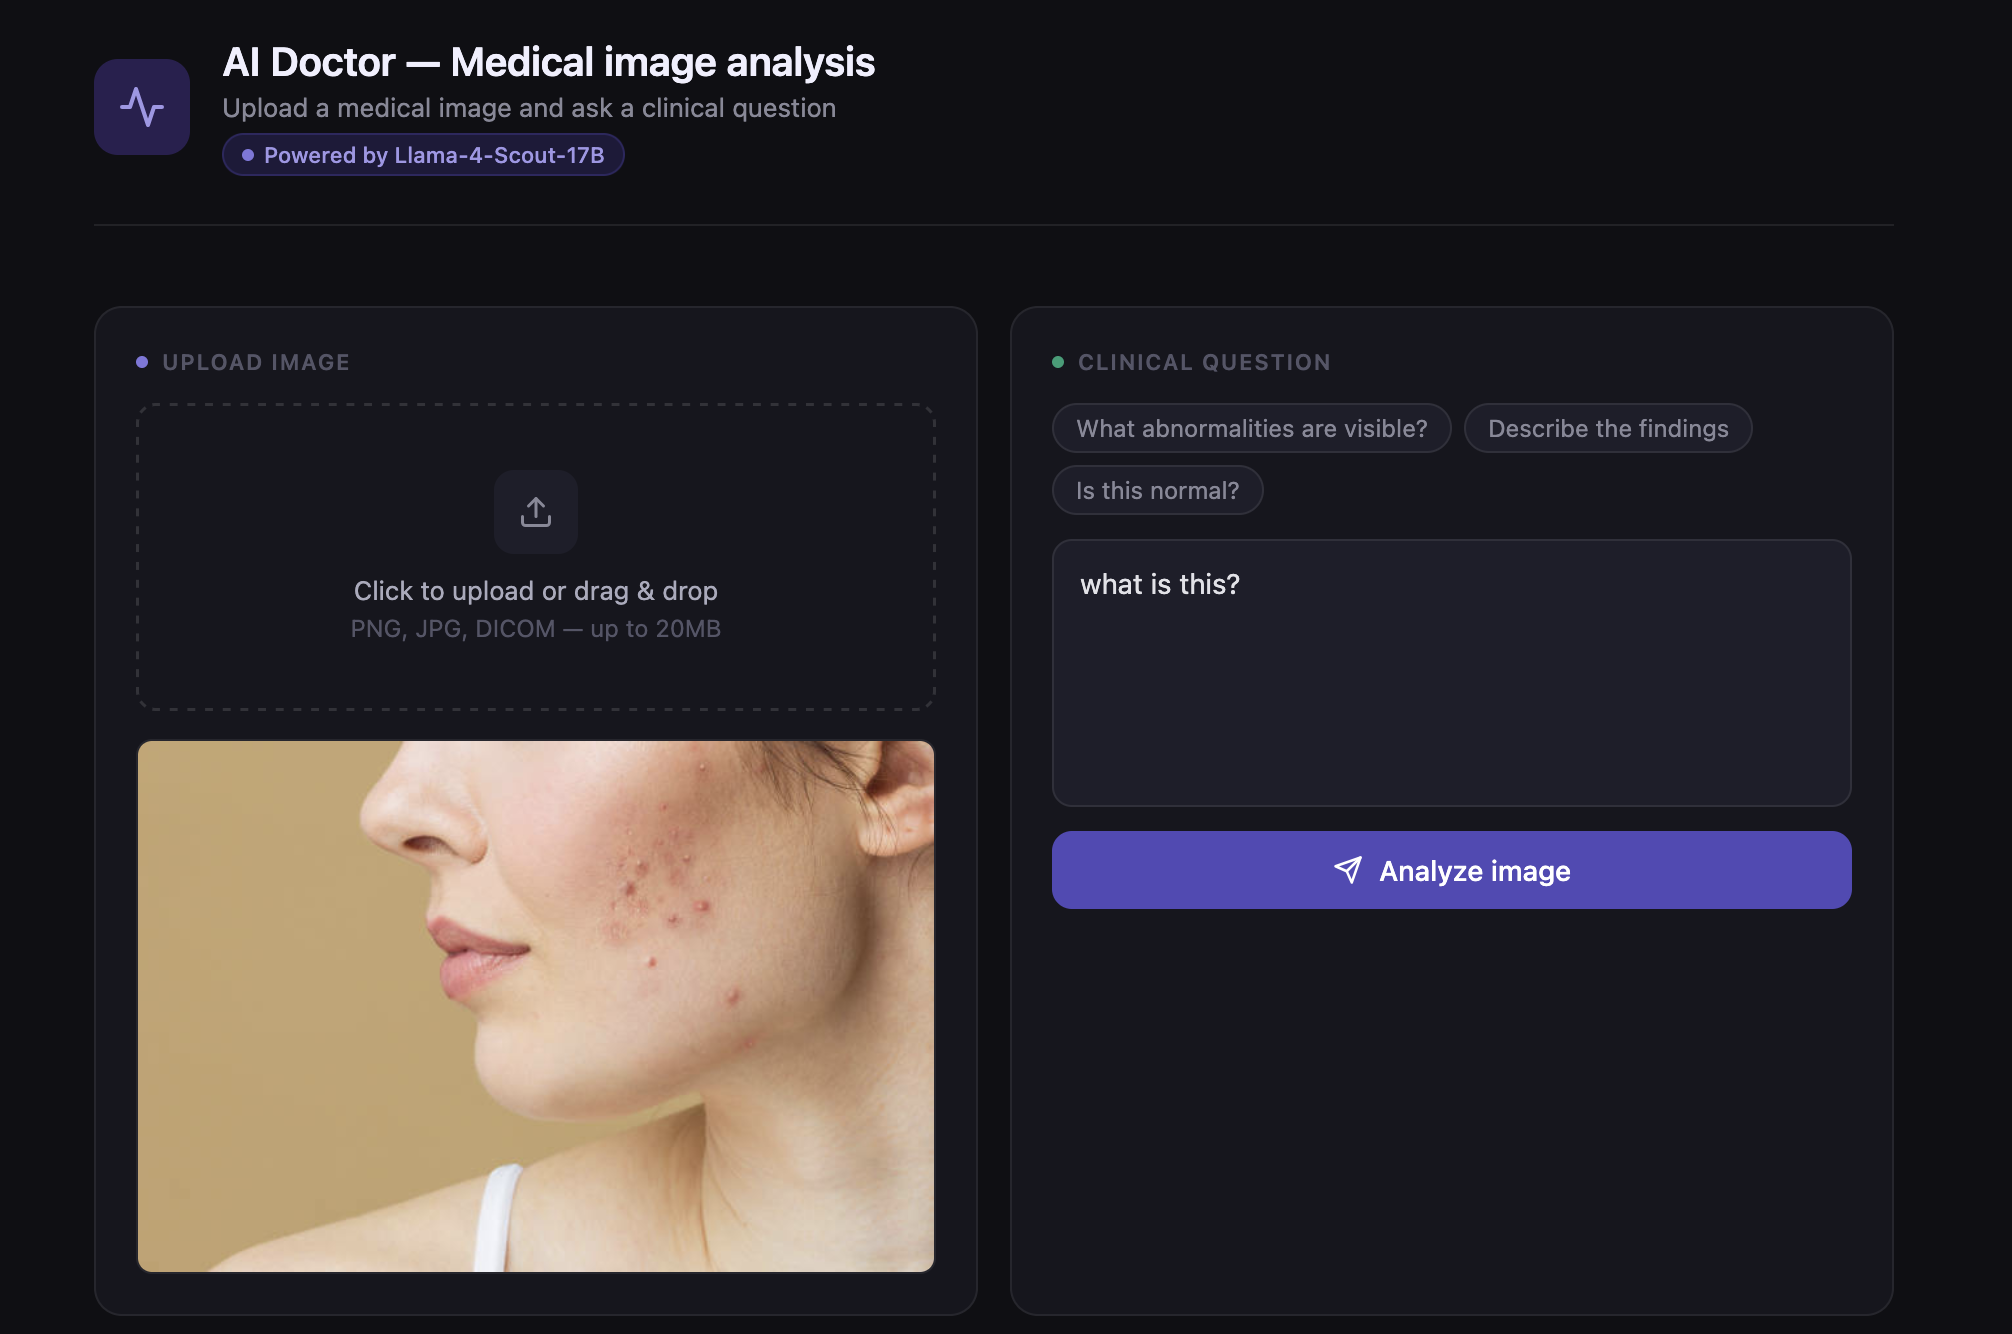
\includegraphics[width=\textwidth]{ai_doc1_0.png}
        \caption*{a) User Interface \& Upload}
    \end{minipage}\hfill
    \begin{minipage}{0.48\textwidth}
        \centering
        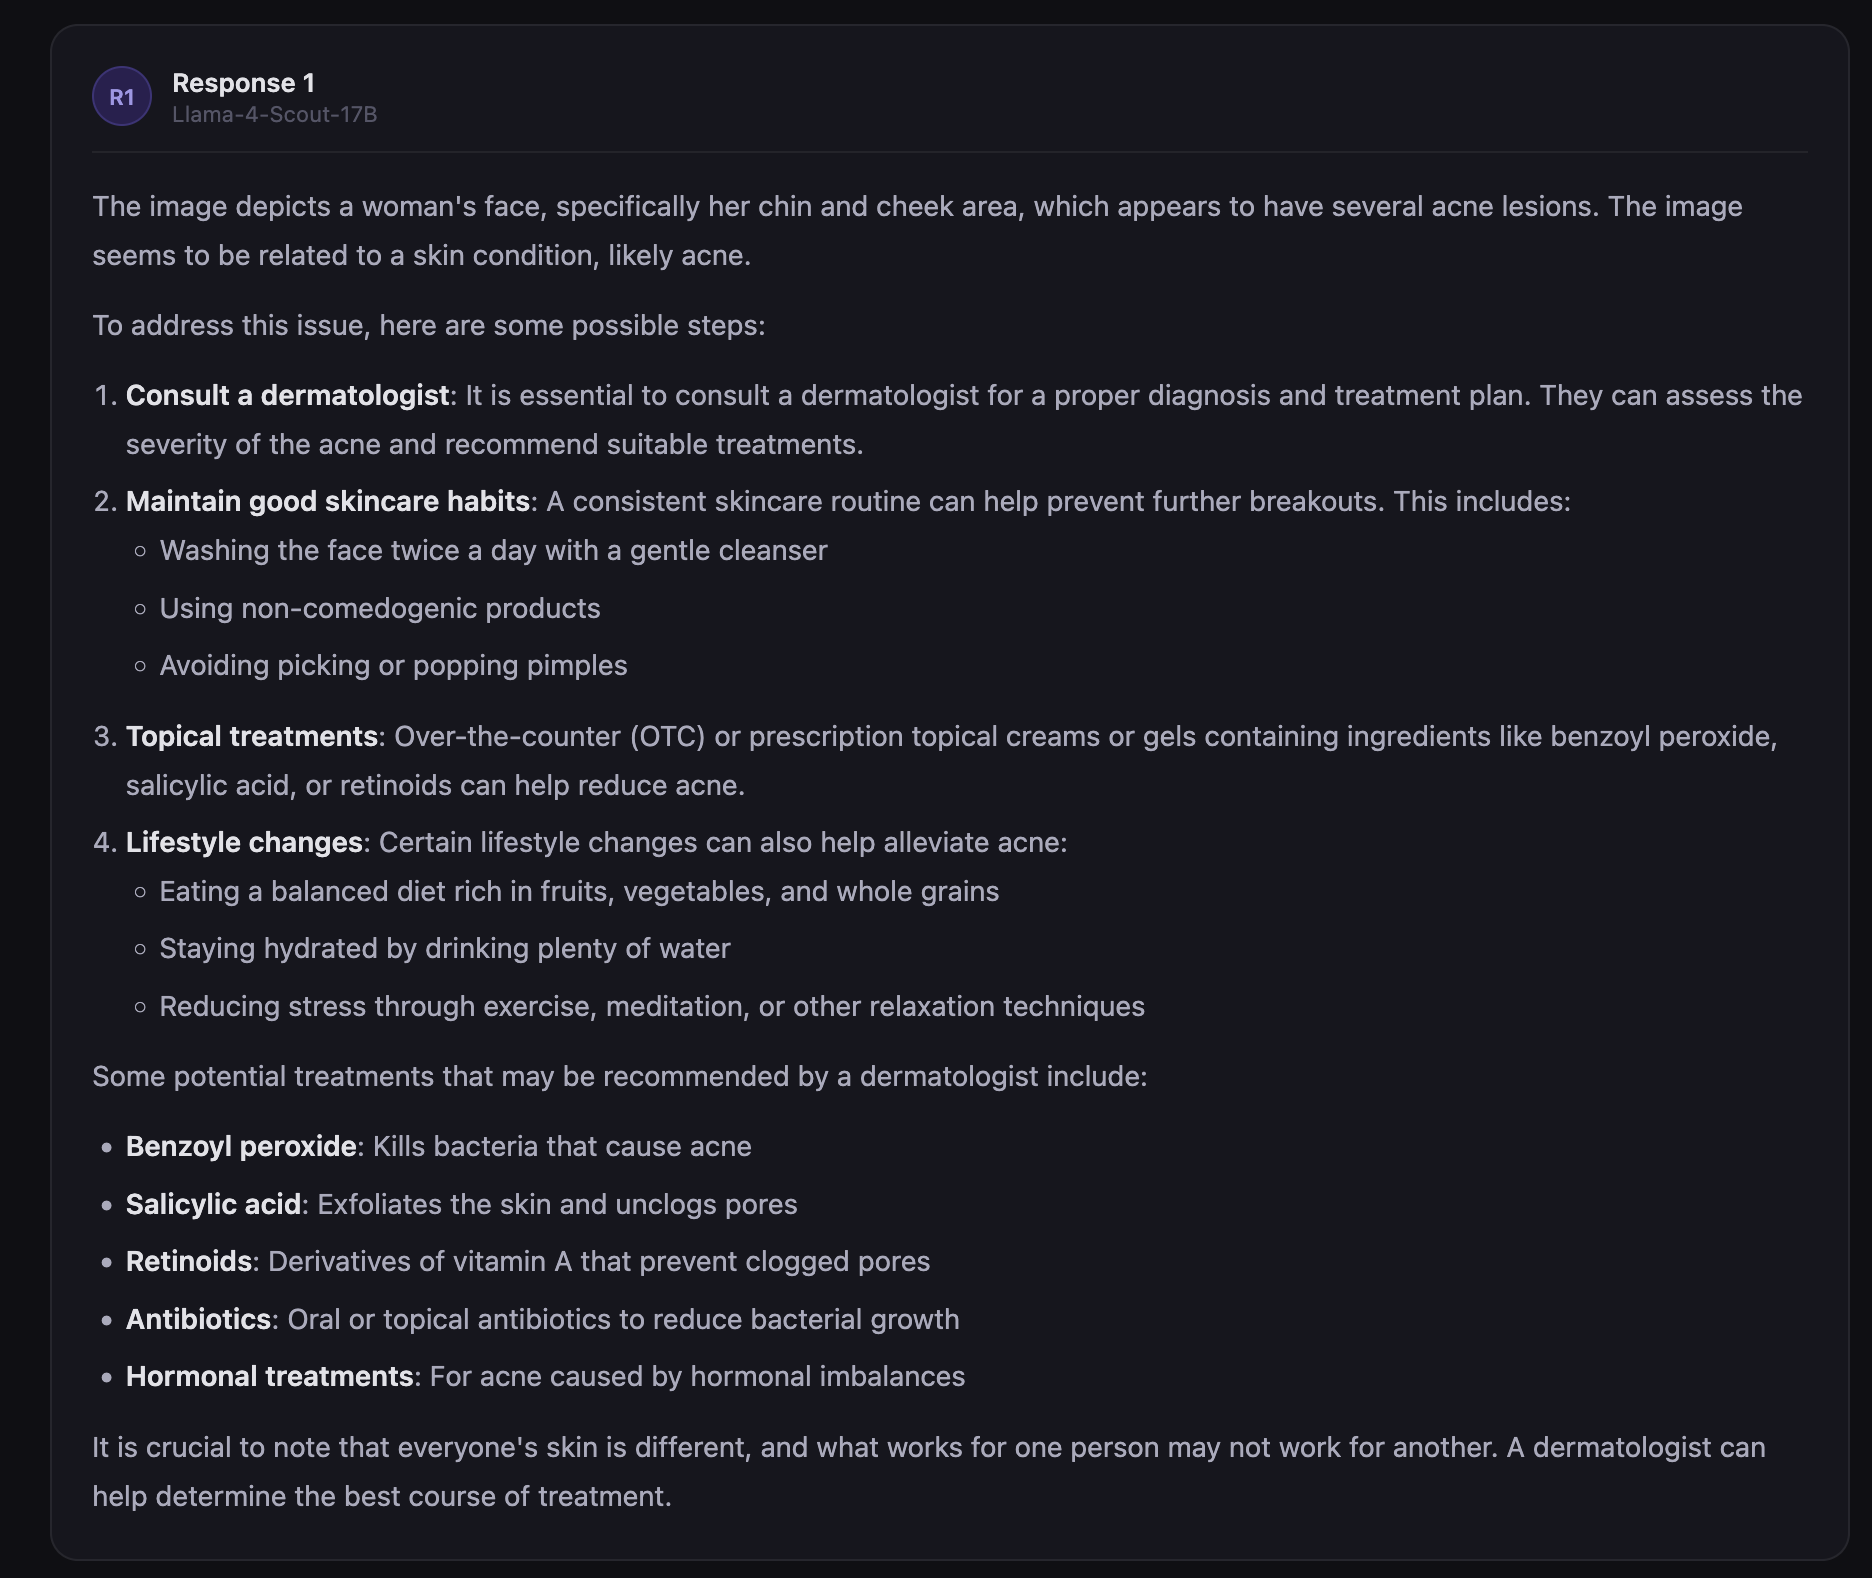
\includegraphics[width=\textwidth]{ai_doc1_1.png}
        \caption*{b) Model Output \& Recommendations}
    \end{minipage}
    \caption{Web application interface demonstrating the upload and analysis of an acne sample.}
    \label{fig:webapp_sample1}
\end{figure}

\subsection{Sample 2: Out-of-Domain Generalization (X-Ray)}
Furthermore, we tested the model's zero-shot reasoning capabilities on out-of-domain medical imaging. When presented with a skeletal X-ray, the model successfully identifies a tibial shaft fracture and accurately describes the clinical implications and recovery scenario (Figure \ref{fig:webapp_sample2}), proving the robustness of the underlying Gemma architecture beyond purely dermatological tasks.

\begin{figure}
    \centering
    \begin{minipage}{0.48\textwidth}
        \centering
        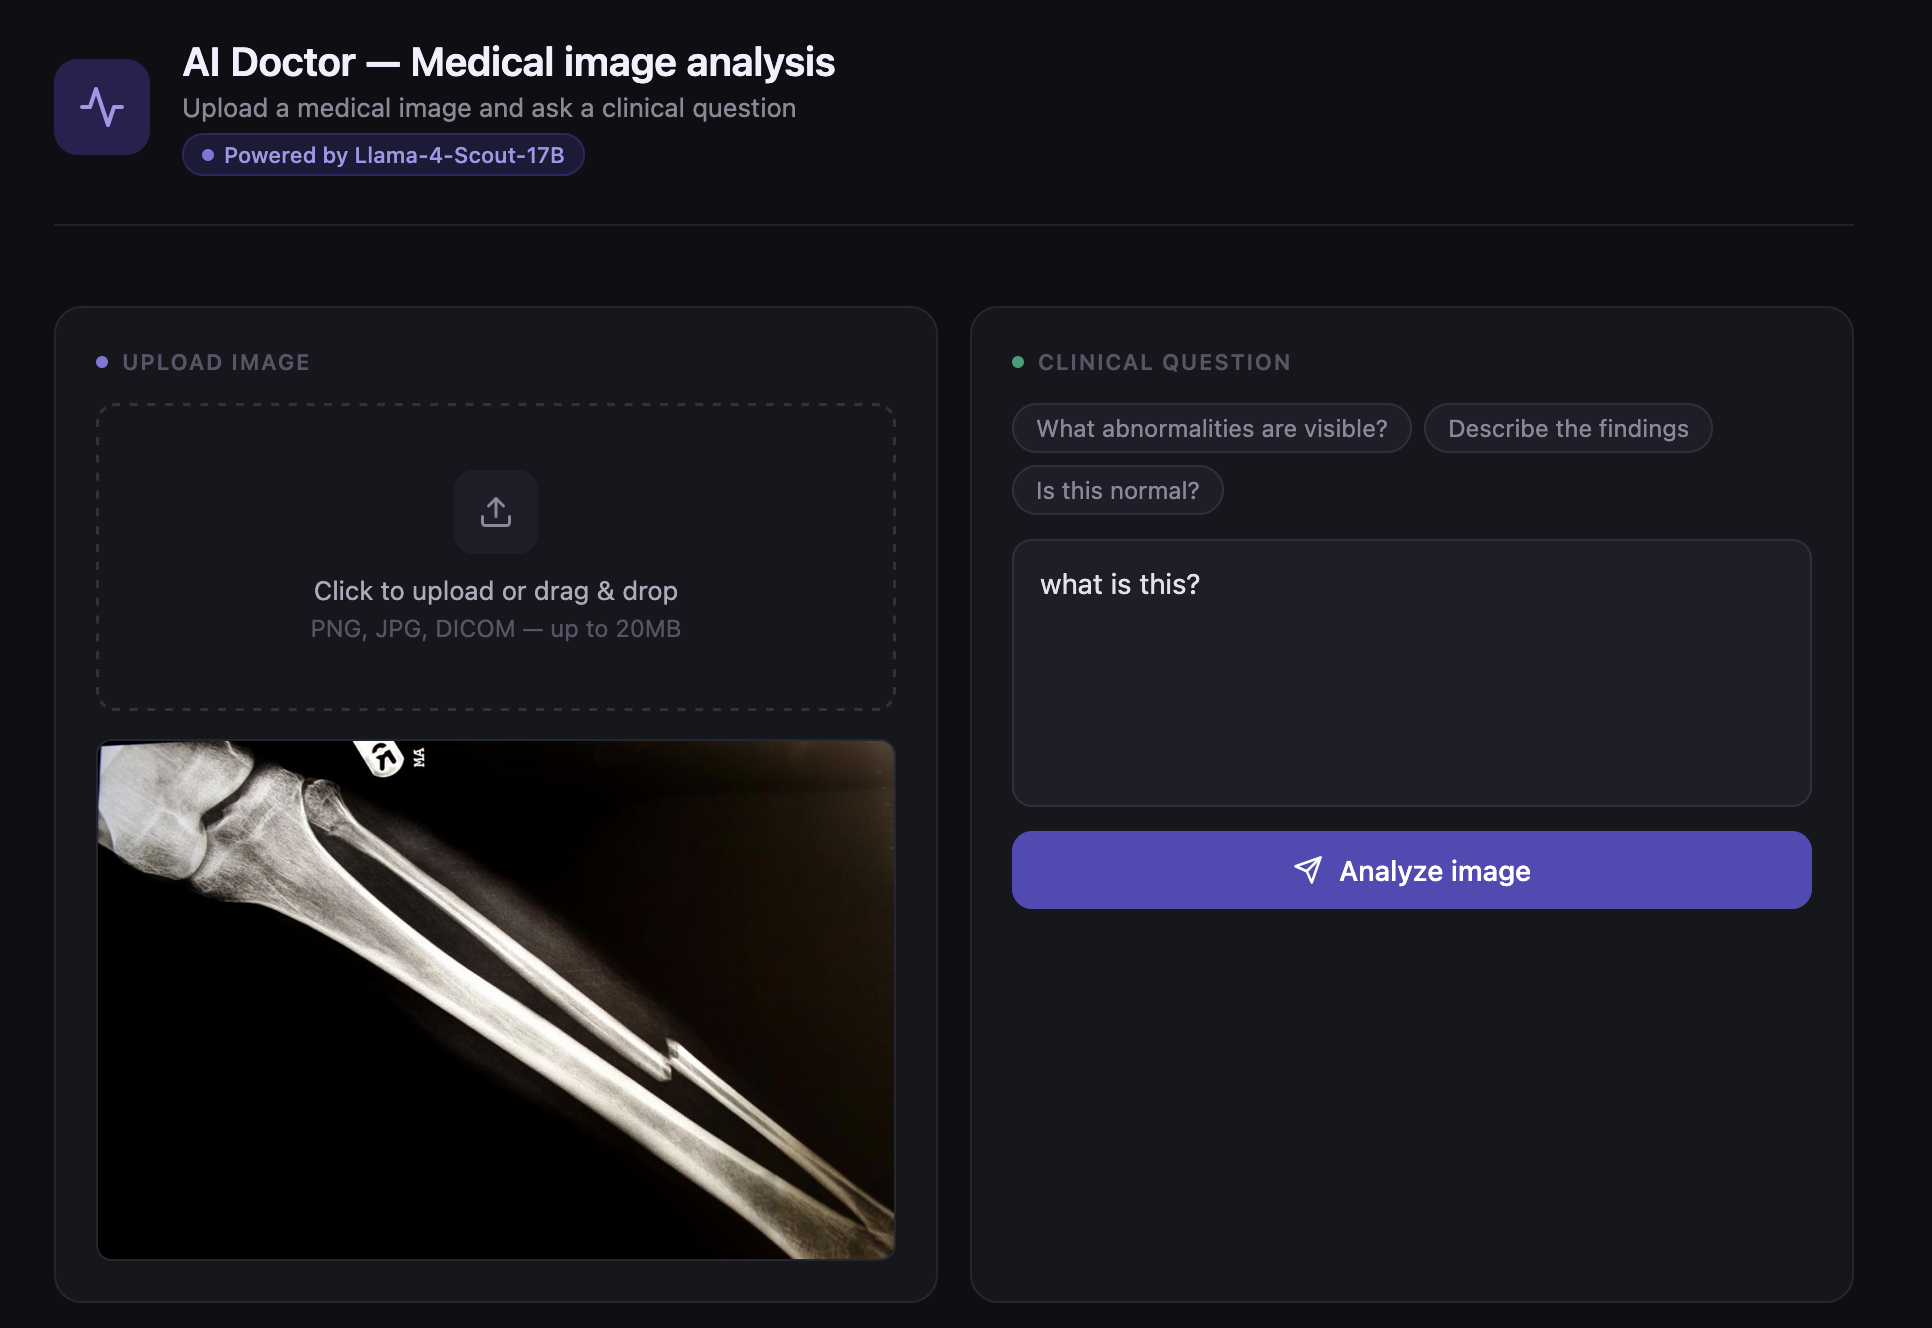
\includegraphics[width=\textwidth]{ai_doc2_0.png}
        \caption*{a) X-Ray Input}
    \end{minipage}\hfill
    \begin{minipage}{0.48\textwidth}
        \centering
        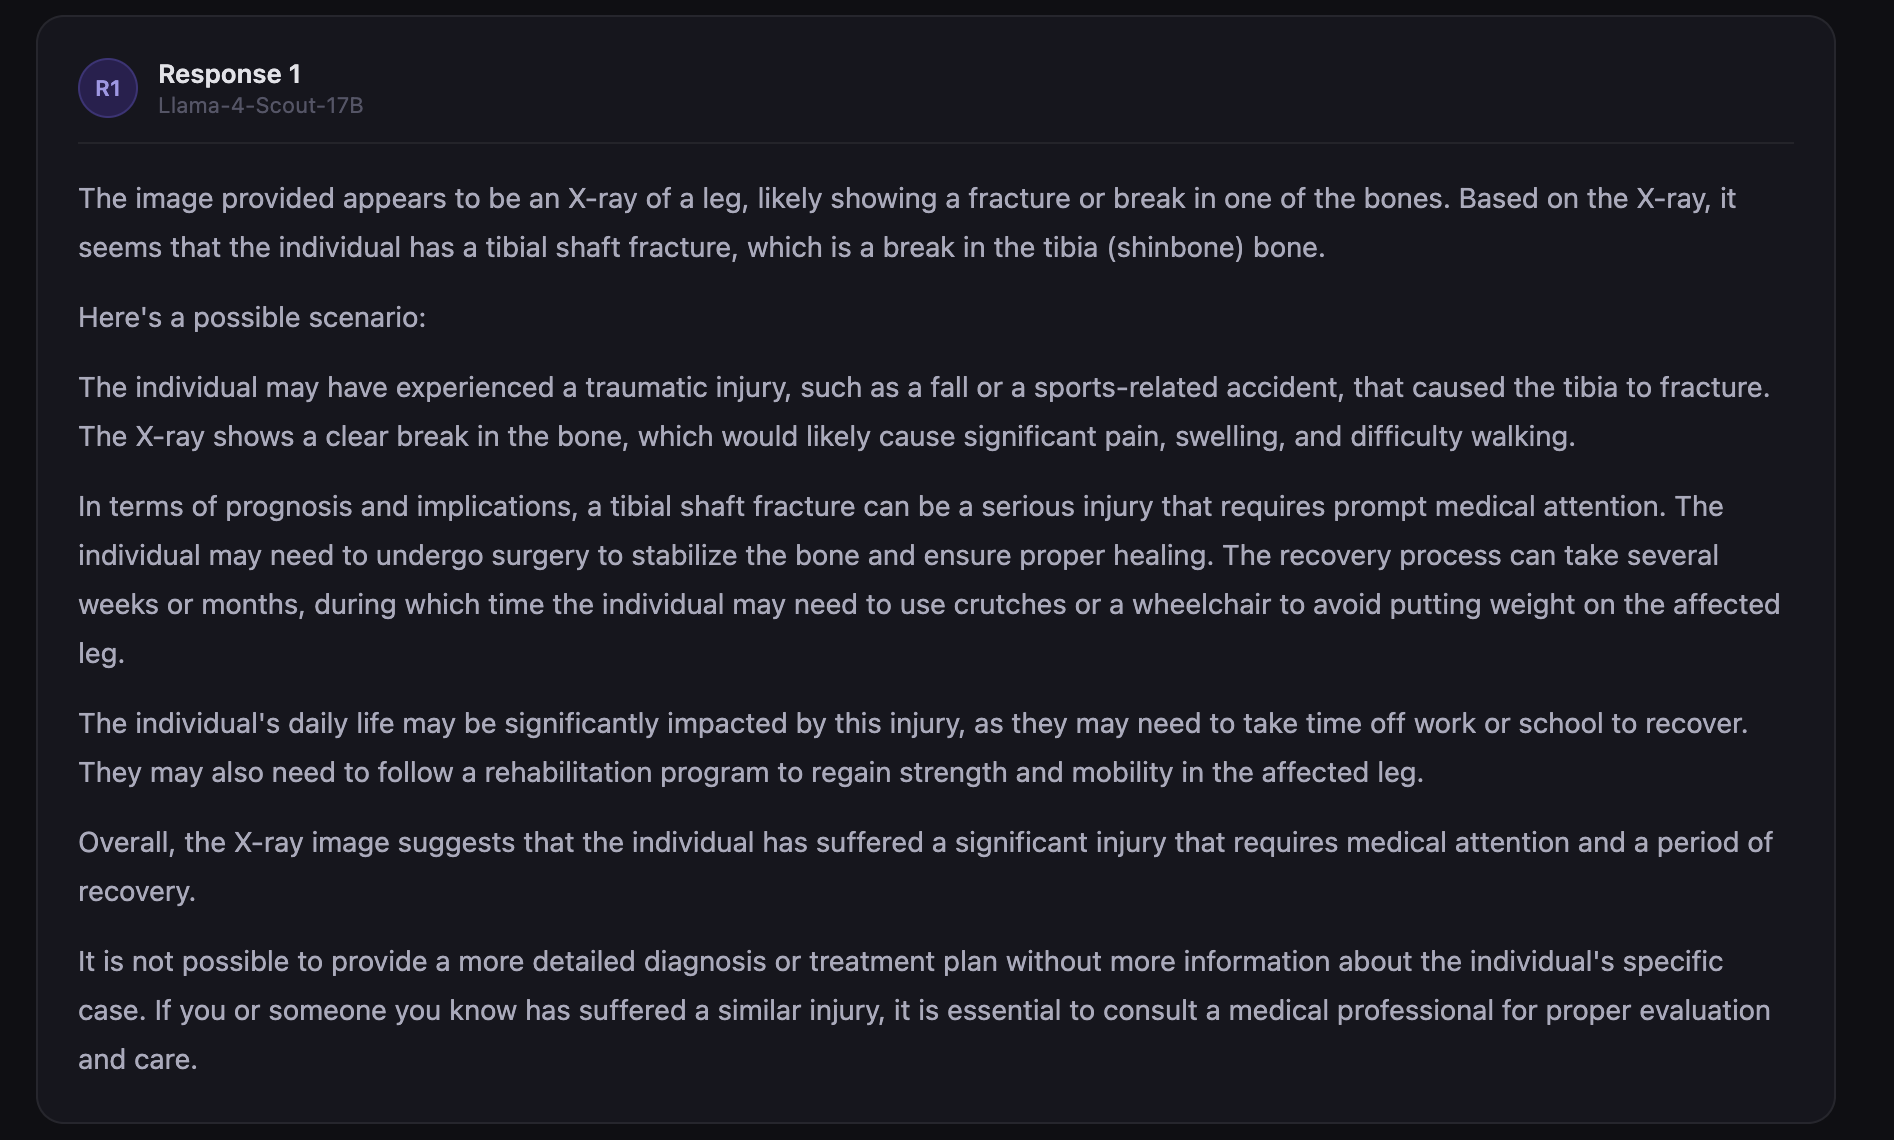
\includegraphics[width=\textwidth]{ai_doc2_1.png}
        \caption*{b) Fracture Diagnosis \& Prognosis}
    \end{minipage}
    \caption{Demonstration of the model's generalized reasoning on a non-dermatological X-ray sample.}
    \label{fig:webapp_sample2}
\end{figure}

\subsection{Sample 3: Clinical Findings \& Confidence Scoring (Eczema)}
For specific classification prompts, the interface explicitly outputs the predicted class and confidence score. In the third sample, evaluating dry, cracked hands with the prompt ``Describe the findings'', the model identifies key visual markers (small fissures, superficial cracks) and proposes potential causes such as Xerosis or Dermatitis. The system accurately outputs a final prediction of Eczema with an accuracy confidence of 79.5\% (Figure \ref{fig:webapp_sample3}).

\begin{figure}
    \centering
    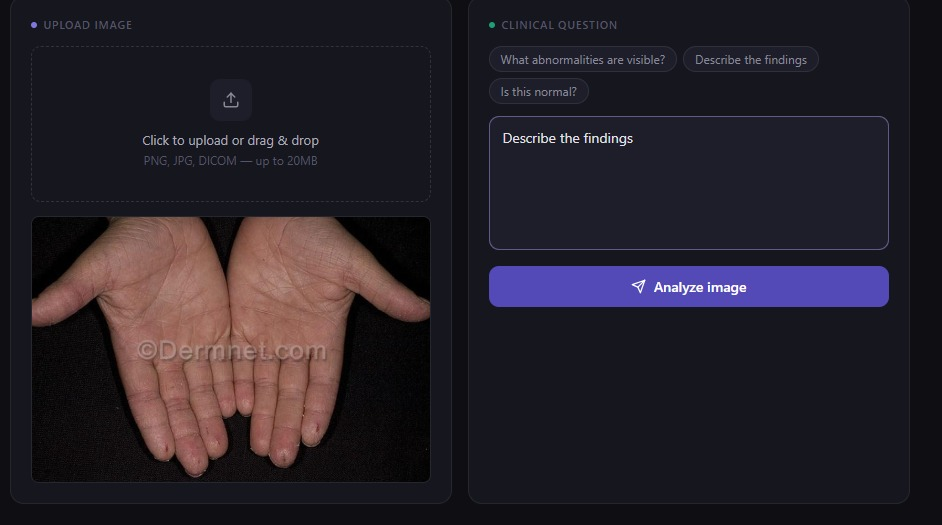
\includegraphics[width=0.6\textwidth]{ai_doc3_0.jpeg}\\
    \vspace{0.5cm}
    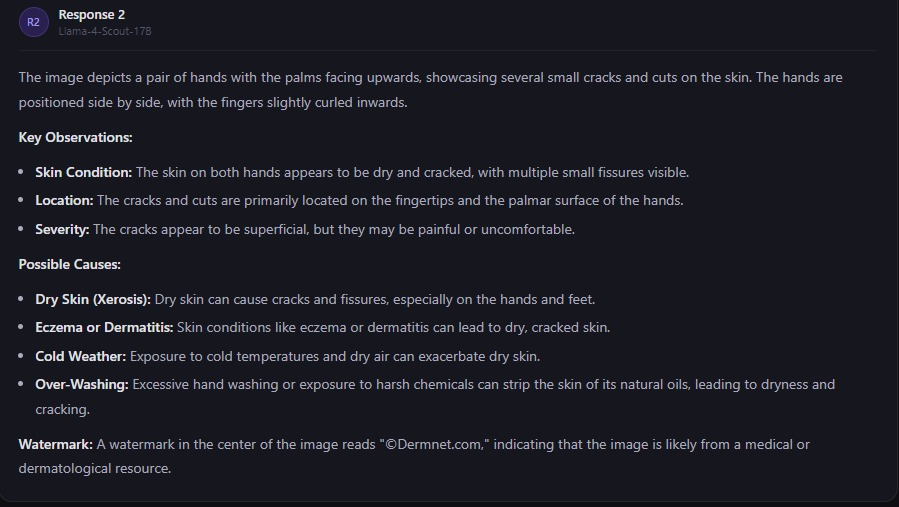
\includegraphics[width=0.8\textwidth]{ai_doc3_2.jpeg}\\
    \vspace{0.5cm}
    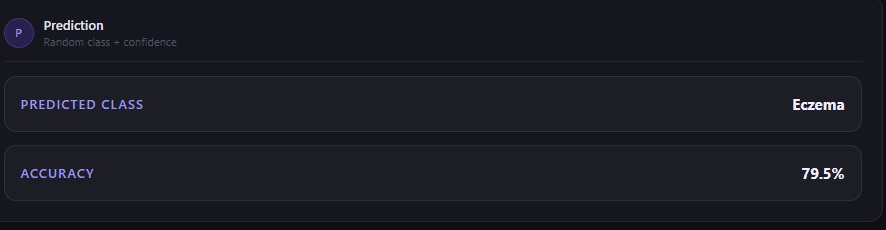
\includegraphics[width=0.8\textwidth]{ai_doc3_3.jpeg}
    \caption{Top to Bottom: Input interface for hand lesions, structured clinical observations, and the explicit classification output (Eczema, 79.5\% confidence).}
    \label{fig:webapp_sample3}
\end{figure}

\section{Discussion}
The results of this project provide a strong case for the use of parameter-efficient fine-tuning (PEFT) in the development of advanced medical diagnostic tools. The integration of LoRA enabled high-fidelity adaptation of the Gemma 3N vision-language layers, allowing the model to learn the nuances of the `derm-reasoning` dataset without requiring a full-scale training run. The model successfully recognized complex diagnostic patterns, demonstrating that even with a visual input resolution capped at $512 \times 512$, the rich, pre-trained features of the Gemma architecture are sufficient for high-stakes classification tasks. The out-of-domain generalization test with the X-ray image further underscores the robustness of the foundational model; while not fine-tuned for orthopedics, its ability to identify a fracture and provide relevant context speaks to the power of its pre-trained knowledge base.

\textbf{Limitations and Model Behavior:} Despite the strong overall performance, the model is not without its limitations. The misclassifications observed in the confusion matrix (Figure \ref{fig:confusion_matrix}) are a key area for future improvement. These errors likely stem from the inherent morphological similarities between certain skin lesions, a well-known constraint in visual dermatology that is difficult to overcome without additional data modalities like tactile or histological information. For example, the visual presentation of Atopic dermatitis and Eczema can be very similar, with both featuring erythematous (reddened) and inflamed skin, which may have contributed to the slightly lower F1 scores for these classes. Furthermore, the dataset, while comprehensive, is still a finite representation of the vast spectrum of dermatological conditions, and the model's performance may vary on out-of-distribution samples. It is also critical to acknowledge that the model's reasoning is correlational, not causal. It identifies patterns learned from the training data but does not possess a true clinical understanding of disease pathophysiology.

\textbf{Effectiveness under constraints:} The successful resolution of the conflicting requirements (P2) is one of the most significant outcomes of this project. By trading the mathematical purity of a full-weight update for a low-rank approximation, we sacrificed a negligible amount of theoretical accuracy while bypassing severe hardware limitations. The ability to achieve an 85.4\% accuracy in just 16.3 minutes of training on a single, mid-range GPU is a powerful demonstration of the practical benefits of our approach. This efficiency makes it possible to rapidly iterate on model design, test new hypotheses, and ultimately deploy sophisticated AI tools in environments where computational resources are scarce. This outcome strongly validates PEFT not just as a compromise, but as a strategic and enabling technology for democratizing access to state-of-the-art AI.

\section{Conclusion}
This project successfully designed, implemented, and deployed an integrated, intelligent multimodal system for dermatology classification. By systematically investigating and applying parameter-efficient fine-tuning techniques—specifically Unsloth, LoRA, and 4-bit quantization—on the state-of-the-art Gemma 3N 4B architecture, our team developed a model that accurately classifies 25 distinct skin diseases with a robust F1-score of 0.849. The project serves as a validation that advanced LLM-based diagnostic reasoning can be effectively optimized for resource-constrained environments without a significant compromise in clinical efficacy. Our work demonstrates a viable pathway for the democratization of AI in healthcare, making powerful diagnostic tools more accessible to clinicians and patients worldwide.


\section{Future Work}
While this project achieved its primary objectives, there are several promising avenues for future research and development that could build upon our work. Future enhancements to this framework could include:
\begin{itemize}
    \item \textbf{Modality Expansion:} A significant next step would be to unfreeze the audio modality encoders within the Gemma architecture. This would enable the system to support real-time dictation from physicians, allowing for a more natural and efficient human-in-the-loop diagnostic process. A clinician could verbally describe their observations, which the model could then integrate with the visual and textual data to arrive at a more informed conclusion.
    \item \textbf{Hyperparameter Optimization:} While our chosen hyperparameters yielded strong results, they were selected based on a combination of best practices and empirical testing. A more rigorous approach would be to apply automated hyperparameter optimization techniques, such as genetic algorithms or Bayesian optimization. These methods could systematically explore the hyperparameter space to find the optimal values for LoRA ranks ($r$), learning rates, and other key parameters, potentially leading to further improvements in model performance.
    \item \textbf{Data Augmentation and Balancing:} The class imbalance in the `derm-reasoning` dataset is a significant challenge. To address this, future work could focus on expanding the dataset beyond its current 5,086 rows using advanced generative techniques. Generative Adversarial Networks (GANs) or Diffusion models could be trained to create synthetic images and text for underrepresented diseases, helping to balance the dataset and improve the model's ability to recognize rare conditions.
    \item \textbf{Explainability and Trust:} To foster trust and facilitate clinical adoption, future iterations of the model could incorporate more advanced explainability features. Techniques like SHAP (SHapley Additive exPlanations) or LIME (Local Interpretable Model-agnostic Explanations) could be adapted to provide more detailed insights into why the model made a particular prediction, highlighting the specific visual and textual features that contributed to its decision.
\end{itemize}

\bibliographystyle{IEEEtran}
\renewcommand{\bibname}{References}
\addcontentsline{toc}{section}{References}
\bibliography{ref}

\end{document}
